\documentclass[12pt]{article}
\usepackage{amsmath,amsfonts,amssymb,fancyhdr,tikz,pgf}
\usetikzlibrary{arrows,positioning,automata}
\pagestyle{fancy}
\usepackage[margin=0.5in]{geometry}
\rhead{$\>$\\*$\>$\\*$\>$\\*Jay LeCavalier - Computer Aided Verification - Midterm Writeup}

\begin{document}
$\>$\\*\\*
\textbf{Problem 2.} $\forall i((0\leq i<N)\rightarrow(p_i\wedge q_i))\rightarrow\forall i((0\leq i\leq2N)\rightarrow(x_0\leq x_i))$ holds for every $N\in\mathbb{N}$\\*\\*
\textit{Proof}: We prove this statement using induction on $N$.\\*\\*
\textit{Basis}: For the basis of induction, we establish that $\forall i((0\leq i<0)\rightarrow(p_i\wedge q_i))\rightarrow\forall i((0\leq i\leq 0)\rightarrow(x_0\leq x_i))$. The antecedent of this conditional is vacuously true, since $0\leq i<0$ is false for any $i\in\mathbb{N}$. Therefore, it will suffice to prove that the consequent, $\forall i((0\leq i\leq 0)\rightarrow(x_0\leq x_i))$, is true. Suppose that $0\leq m\leq0$. Then $m=0$. Consequently, $x_0\leq x_m$ holds trivially, because $x_0\leq x_0$. Thus, the theorem holds when $N=0$.\\*\\*
\textit{IH}: For the induction hypothesis, suppose that $\forall i((0\leq i<N)\rightarrow(p_i\wedge q_i))\rightarrow\forall i((0\leq i\leq2N)\rightarrow(x_0\leq x_i))$.\\*\\*
\textit{IS}: Suppose that $\forall i((0\leq i<N+1)\rightarrow p_i\wedge q_i))$. Furthermore, suppose that $0\leq m\leq2(N+1)$. Either $m<N+1$ or $m\geq N+1$. We consider each case in detail:\\*\\*
i) If $m<N+1$, then, since $\forall i((0\leq i<N+1)\rightarrow p_i\wedge q_i))$ holds by assumption, we must have $\forall i((0\leq i<N)\rightarrow p_i\wedge q_i))$ trivially. Since $\forall i((0\leq i<N)\rightarrow p_i\wedge q_i))$, $\forall i((0\leq i\leq2N)\rightarrow(x_0\leq x_i))$ holds by the \textit{IH}. Since $0\leq m<N+1$, we must have $0\leq m\leq2N$. Therefore, because $0\leq m\leq2N$ and $\forall i((0\leq i\leq2N)\rightarrow(x_0\leq x_i))$, we have $x_0\leq x_m$.\\*\\*
ii) If $m\geq N+1$, then it is easy to check that either $m=2i+1$ or $m=2i+2$ for some $i<N+1$. Since $i<N+1$, $p_i\wedge q_i$ by our initial supposition. If $m=2i+1$, then, since $p_i$ holds, $x_{2i}\leq x_m$. If $m=2i+2$, then, since $q_i$ holds, $x_{2i}\leq x_m$ as well. Thus, in either of our two cases, $x_{2i}\leq x_m$. Since $i<N+1$, $2i\leq2N$ trivially, which means that $x_0\leq x_{2i}$ by the \textit{IH}. Since $x_0\leq x_{2i}$ and $x_{2i}\leq x_m$, we must have $x_0\leq x_m$.\\*\\*
In both of the two cases, (i) and (ii), we see that $x_0\leq x_m$, which means that $\forall i((0\leq i\leq2(N+1))\rightarrow(x_0\leq x_i))$.$\hfill\Box$\\*\\*
\textbf{Problem 3.} $\forall i((i\geq0)\rightarrow(p_i\wedge q_i))$ is inductive.\\*\\*
\textit{Proof}: We have already shown that $\forall i((i\geq0)\rightarrow p_i)$ is inductive, so we must prove the same thing for the predicate $q$.\\*\\*
Suppose that in a certain state, we satisfy $\forall i((i\geq0)\rightarrow(p_i\wedge q_i))$. Suppose that $i\geq0$. Then, $q_i$ holds by supposition, which means that $x_{2i}\leq x_{2i+2}$. Now, suppose that we transition to a new state. We want to show that in this new state, $x^\prime_{2i}\leq x^\prime_{2i+2}$. This transition was either a push or a pop. We consider each case:\\*\\*
i) If the transition was a push, $x^\prime_{2i}=min(x_{2i},x_{2i-1})$ and $x^\prime_{2i+2}=x^\prime_{2(i+1)}=min(x_{2i+2},x_{2i+1})$. So, we want to show that $min(x_{2i},x_{2i-1})\leq min(x_{2i+2},x_{2i+1})$. This gives us four more sub-cases:\\*\\*
a) First of all, $x_{2i}\leq x_{2i+2}$ by the fact that $q_i$ holds. Therefore, if $min(x_{2i},x_{2i-1})=x_{2i}$ and $min(x_{2i+2},x_{2i+1})=x_{2i+2}$, then $min(x_{2i},x_{2i-1})\leq min(x_{2i+2},x_{2i+1})$.\\*
b) Now, if $min(x_{2i},x_{2i-1})=x_{2i-1}$ and $min(x_{2i+2},x_{2i+1})=x_{2i+2}$, then $x_{2i-1}\leq x_{2i}$ trivially. We have already seen from case (a) that $x_{2i}\leq x_{2i+2}$. Since $x_{2i}\leq x_{2i+2}$ and $x_{2i-1}\leq x_{2i}$, we must have $x_{2i-1}\leq x_{2i+2}$, which means $min(x_{2i},x_{2i-1})\leq min(x_{2i+2},x_{2i+1})$.\\*
c) Since $p$ is an inductive property, we must have $x_{2i}\leq x_{2i+1}$. Therefore, if $min(x_{2i},x_{2i-1})=x_{2i}$ and $min(x_{2i+2},x_{2i+1})=x_{2i+1}$, then $min(x_{2i},x_{2i-1})\leq min(x_{2i+2},x_{2i+1})$.\\*
d) Finally, $x_{2i-1}\leq x_{2i+1}$, since $q$ holds by supposition. Therefore, if $min(x_{2i},x_{2i-1})=x_{2i-1}$ and $min(x_{2i+2},x_{2i+1})=x_{2i+1}$, then $min(x_{2i},x_{2i-1})\leq min(x_{2i+2},x_{2i+1})$.\\*\\*
In all four cases, we showed that $x^\prime_{2i}\leq x^\prime_{2i+2}$, which means that $q_i$ is an inductive property across all push operations.\\*\\*
ii) If the transition was a pop, then we want to show that $min(x_{2i+1},x_{2i+2})\leq min(x_{2i+3},x_{2i+4})$. Again, we can split this up into four sub-cases:\\*\\*
a) First of all, $x_{2i+2}\leq x_{2i+3}$ since $p_i$ holds by assumption, so if $min(x_{2i+1},x_{2i+2})=x_{2i+2}$ and $min(x_{2i+3},x_{2i+4})=x_{2i+3}$, then $min(x_{2i+1},x_{2i+2})\leq min(x_{2i+3},x_{2i+4})$.\\*
b) Also, $x_{2i+2}\leq x_{2i+4}$ since $q_i$ holds by assumption, so if $min(x_{2i+1},x_{2i+2})=x_{2i+2}$ and $min(x_{2i+3},x_{2i+4})=x_{2i+4}$, then $min(x_{2i+1},x_{2i+2})\leq min(x_{2i+3},x_{2i+4})$.\\*
c) If $min(x_{2i+1},x_{2i+2})=x_{2i+1}$ and $min(x_{2i+3},x_{2i+4})=x_{2i+4}$, then $x_{2i+1}\leq x_{2i+2}$. We already showed in case (b) that $x_{2i+2}\leq x_{2i+4}$, so this means that $x_{2i+1}\leq x_{2i+2}$. Thus, $min(x_{2i+1},x_{2i+2})\leq min(x_{2i+3},x_{2i+4})$.\\*
d) Finally, if $min(x_{2i+1},x_{2i+2})=x_{2i+1}$ and $min(x_{2i+3},x_{2i+4})=x_{2i+3}$, then again we have $x_{2i+1}\leq x_{2i+2}$. In case (a) we showed $x_{2i+2}\leq x_{2i+3}$, so $x_{2i+1}\leq x_{2i+3}$. Therefore, $min(x_{2i+1},x_{2i+2})\leq min(x_{2i+3},x_{2i+4})$ in this case as well.\\*\\*
Whether we push or pop, the property $q$ is preserved. Since $p_i\wedge q_i$ holds at the initial state and $p_i\wedge q_i$ holds at every state we can transition into from a state satisfying $p_i\wedge q_i$, we conclude that the property is inductive.$\hfill\Box$\\*\\*
\textbf{Problem 4.} First, we expand the formula $\varphi=pRFq$ into disjunctive normal form:\\*\\*
$pRFq\Longleftrightarrow Fq\wedge(p\vee X(pRFq))$\\*
$Fq\wedge(p\vee X(pRFq))\Longleftrightarrow(q\vee X(Fq))\wedge(p\vee X(pRFq))$\\*
$(q\vee X(Fq))\wedge(p\vee X(pRFq))\Longleftrightarrow(p\wedge q)\vee(p\wedge X(Fq))\vee(q\wedge X(pRFq))\vee(X(Fq)\wedge X(pRFq))$\\*
$\Longleftrightarrow(p\wedge q\wedge X(true))\vee(p\wedge X(Fq))\vee(q\wedge X(pRFq))\vee(true\wedge X(Fq\wedge pRFq))$\\*\\*
Now, we can create the corresponding Buchi automata:\\*\\*
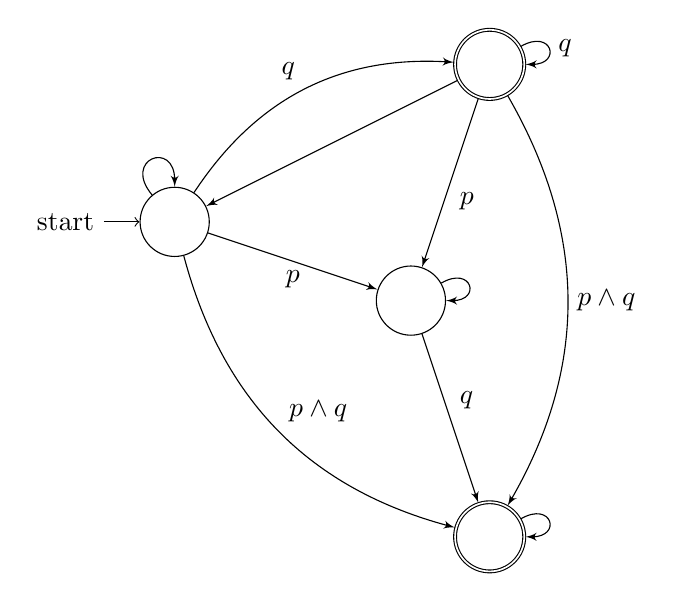
\begin{tikzpicture}
\tikzset{vertex/.style = {shape=circle,draw,minimum size=1.5em}}
\tikzset{edge/.style = {->,> = latex'}}
% NODES
\node[state][initial] (a) at (0,0) {};
\node[state] (b) at (3,-1) {};
\node[state][accepting] (c) at (4,2) {};
\node[state][accepting] (d) at (4,-4) {};
% EDGES
\draw[edge][loop][in=90,out=130,looseness=5] (a) to (a);
\draw[edge] (a) to node [auto,below] {$p$} (b);
\draw[edge][bend left] (a) to node [auto] {$q$} (c);
\draw[edge][bend right] (a) to node [auto] {$p\wedge q$} (d);

\draw[edge] (b) to node [auto] {$q$} (d);
\draw[edge][loop][in=0,out=30,looseness=5] (b) to (b);

\draw[edge] (c) to node [auto] {} (a);
\draw[edge] (c) to node [auto] {$p$} (b);
\draw[edge][bend left] (c) to node [auto] {$p\wedge q$} (d);
\draw[edge][loop][in=0,out=30,looseness=5] (c) to node [auto,right] {$q$} (c);

\draw[edge][loop][in=0,out=30,looseness=5] (d) to (d);
\end{tikzpicture}\\*\\*
\textbf{Problem 5.}
\end{document}